%
% firmware.tex
%
% Copyright (C) 2019 by Universidade Federal de Santa Catarina.
%
% OBDH 2.0 Documentation
%
% This work is licensed under the Creative Commons Attribution-ShareAlike 4.0
% International License. To view a copy of this license,
% visit http://creativecommons.org/licenses/by-sa/4.0/.
%

%
% \brief Firmware chapter.
%
% \author Gabriel Mariano Marcelino <gabriel.mm8@gmail.com>
%
% \institution Universidade Federal de Santa Catarina (UFSC)
%
% \version 0.1.0
%
% \date 30/10/2019
%

\chapter{Firmware} \label{ch:firmware}

\section{Tasks}

\begin{table}[!h]
    \centering
    \begin{tabular}{lllll}
        \toprule[1.5pt]
        \textit{Name}          & \textit{Priority} & \textit{Initial delay [ms]} & \textit{Period [ms]} \\
        \midrule
        Startup (boot)         & Highest           & 0                           & Aperiodic            \\
        Deployment hibernation & Highest           & 0                           & Aperiodic            \\
        Antenna deployment     & Highest           & 0                           & Aperiodic            \\
        Watchdog reset         & Lowest            & 0                           & 100                  \\
        Periodic downlink      & Medium            & 5000                        & 60000                \\
        Uplink                 & High              & 5000                        & 1000                 \\
        EPS reading            & Medium            & 5000                        & 60000                \\
        EDC reading            & High              & 5000                        & 1000                 \\
        Payload X reading      & Medium            & 5000                        & 5000                 \\
        TTC writing            & Medium            & 5000                        & Beacon period        \\
        Radio periodoc reset   & Low               & 0                           & 600000               \\
        OBDH reset             & Low               & 0                           & 36000000             \\
        \bottomrule[1.5pt]
    \end{tabular}
    \caption{Firmware tasks.}
    \label{tab:firmware-tasks}
\end{table}

\section{Telecommands}

\begin{table}[!h]
    \centering
    \begin{tabular}{lll}
        \toprule[1.5pt]
        \textit{Name}          & \textit{Parameters}           & \textit{Access} \\
        \midrule
        Enter hibernation      & Hibernation period in seconds & Private         \\
        Leave hibernation      & None                          & Private         \\
        Activate beacon        & None                          & Private         \\
        Deactivate beacon      & None                          & Private         \\
        Activate downlink      & None                          & Private         \\
        Deactivate dtownlink   & None                          & Private         \\
        Activate EDC           & None                          & Private         \\
        Deactivate EDC         & None                          & Private         \\
        Activate Payload X     & Experiment period in seconds  & Private         \\
        Deactivate Payload X   & None                          & Private         \\
        Set system time        & Time value (epoch)            & Private         \\
        Ping                   & None                          & Public          \\
        Message broadcast      & ASCII message                 & Public          \\
        Request data           & Data flags                    & Public          \\
        \bottomrule[1.5pt]
    \end{tabular}
    \caption{System telecomamnds.}
    \label{tab:system-telecommands}
\end{table}

\section{Operating System}

FreeRTOS 10

\section{Hardware Abstraction Layer (HAL)}

DriverLib

\section{Protocols}

\subsection{NGHam}

NGHam \cite{ngham}, short for Next Generation Ham Radio, is a set of protocols for packet radio communication. Its usage is similar to the existing AX.25 protocol.

\begin{figure}[!ht]
    \begin{center}
        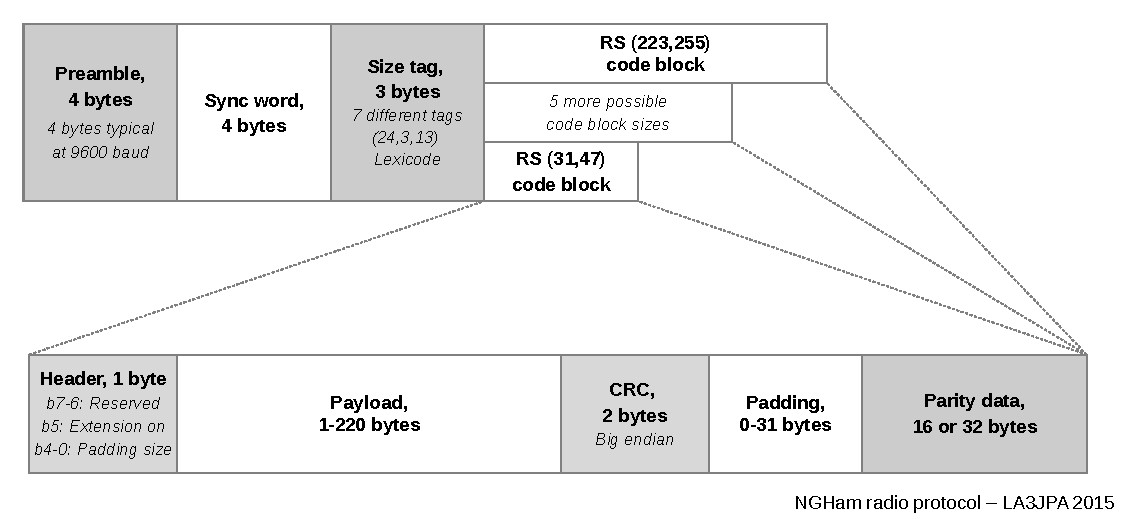
\includegraphics[width=\textwidth]{figures/ngham_block_v4.pdf}
        \caption{NGHam packet structure.}
        \label{fig:ngham-stack}
    \end{center}
\end{figure}
